\chapter{Implementation\label{cha:chapter5}}
A proof of concept implementation of the concept introduced in chapter \ref{cha:chapter4} is documented in this chapter. The code is available here: \url{https://github.com/gurukeuck/Master-s-Thesis}

\section{Requirements}
To run this framework, you need to meet these requirements:
\begin{itemize}
    \item Docker
    \item Python 3+ plus following packages:
    \begin{itemize}
        \item docker
        \item grpcio
        \item protobuf
        \item googleapis-common-protos
        \item opcua
    \end{itemize}
\end{itemize}

\section{Sequence Diagrams and Method Signatures}
The subsections are named like the methods you call during usage. They illustrate the process of a CAD file or camera image to determining the pose of an object inside that file or image. Requirement is having a ready to use detector and camera Docker image loaded in Docker hub and a CAD file. 

The modules have no GUI, instead they are command line based. However, you could use e.g. UA Expert for calling OPC UA Vision methods.

In the diagrams of this section, dashed arrows denote gRPC connections, dotted arrows denote OPC UA connections. Signatures are hidden in the diagrams for a more concise overview. OPC UA and gRPC methods are written in CamelCase, thus the different naming conventions in the implementation.

\subsection{GetConfig}\label{subsec:getconfig}
This optional method can be used to gather the current configuration of the detector or camera docker image. See figure \ref{fig:SequenceDiagram-GetConfig}.

\begin{figure}[ht]
	\centering
  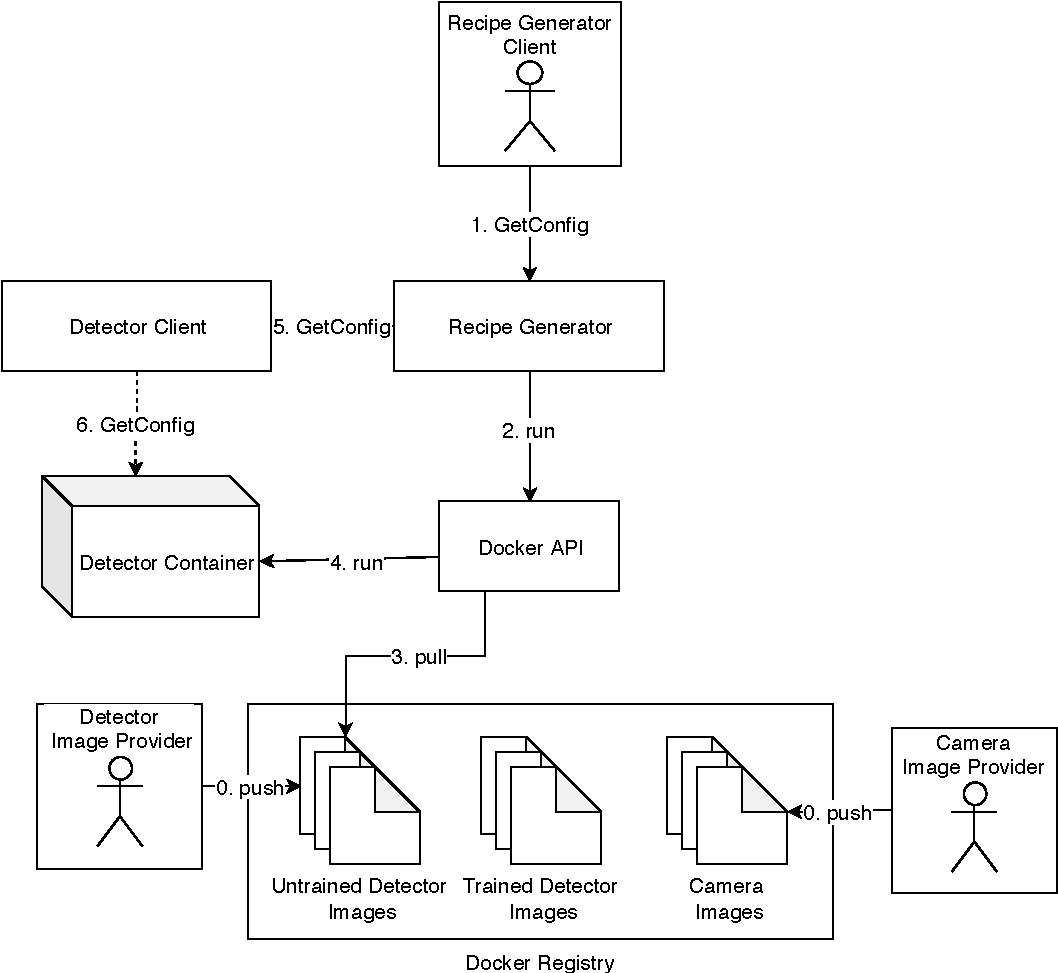
\includegraphics[width=\textwidth]{img/SequenceDiagram-GetConfig.pdf}
	\caption{Sequence Diagram - GetConfig}
	\label{fig:SequenceDiagram-GetConfig}
\end{figure}

\begin{enumerate}
    \item \mintinline{Python}{GetConfig} is called by the recipe generator client which could be a machine operator, a PLC or production planner. \begin{tabbing}
            space \= space \= spacespacespace \= spacespacespacespace \= spacespacespace \kill
            \>  GetConfig(\\
            \>  \>  (out)	 \> 	String           \> Config); 
        \end{tabbing} \label{sign:getconfig}
        
    \item To run this method it is necessary to instantiate an instance of the \mintinline{Python}{DockerApi} class which connects to a Docker registry provided by environment variables. You need to provide an \mintinline{Python}{imageName} when instantiating. Running the \mintinline{Python}{run} method does not require any input, a \mintinline{Python}{port} can be stated optionally (default 8000 for detectors, 8011 for cameras): \begin{tabbing}
    space \= space \= spacespacespace \= spacespacespacespace \= spacespacespace \kill
    \>  run\_container(\\
    \>  \>  (in)	 \> 	Int          \> port\\
    \>  \>  (out)	 \> 	ContainerObject           \> container); 
    \end{tabbing}
    \mintinline{Python}{ContainerObject} will be returned by the nested method call explained in point 4. \label{sign:runcontainer}
    \item Pull method is invoked by the run method in point 4 and needs no calling. \label{sign:pull}
    \item See \cite{LastvisitedMay4th2019DockerPython} for a detailed reference of \mintinline{Python}{run}: 
    \begin{tabbing}
    space \= space \= spacespacespace \= spacespacespacespace \= spacespacespace \kill
    \>  run(\\
    \>  \>  (in)	 \> 	String          \> imageName\\
    \>  \>  (in)	 \> 	boolean          \> detach\\
    \>  \>  (in)	 \> 	boolean    \> autoremove\\
    \>  \>  (in)	 \> 	Dict   \> ports\\
    \>  \>  (in)	 \> 	boolean   \> stderr\\
    \>  \>  (in)	 \> 	boolean          \> stdout\\
    \>  \>  (out)	 \> 	ContainerObject           \> container); 
    \end{tabbing}\label{sign:run}
    \item \mintinline{Python}{GetConfig} is a member of a \mintinline{Python}{DetectorClient} which is initialized with a gRPC channel to the detector and and interfacing stub. GetConfig can be called with no input. For the signature see \ref{sign:getconfig}.
    \item \mintinline{Python}{GetConfig} gathers the config via gRPC. For the signature see  \ref{sign:getconfig} in.
\end{enumerate}


\subsection{Train}
See figure \ref{fig:SequenceDiagram-Train}.
\begin{enumerate}
    \item \mintinline{Python}{Train} uses a CAD file and an optional configuration file as input to train the detector for later usage. It returns the train result and optional camera image files for result representation.
        \begin{tabbing}
        space \= space \= spacespacespace \= spacespacespacespace \= spacespacespace \kill
        \>  Train(\\
        \>  \>  (in)	 \> 	file          \> cad\\
        \>  \>  (in)	 \> 	file          \> conf\\
        \>  \>  (out)	 \> 	file          \> image\\
        \>  \>  (out)	 \> 	String           \> result); 
        \end{tabbing}\label{sign:train}
    \item See point \ref{sign:runcontainer} in \ref{subsec:getconfig}.
    \item See point \ref{sign:pull} in \ref{subsec:getconfig}.
    \item See point \ref{sign:run} in \ref{subsec:getconfig}.
    \item \mintinline{Python}{Train} is a member of a \mintinline{Python}{DetectorClient} which is initialized with a gRPC channel to the detector and and interfacing stub. See point \ref{sign:train} for the signature.
    \item \mintinline{Python}{Train} gathers the config via gRPC. See point \ref{sign:train} for the signature.
    \item \mintinline{Python}{commit} creates an image of the running detector container instance and pushes it to a repository. It is a method part of the Docker Python framework described in \cite{LastvisitedMay4th2019DockerPython}, see a detailed description of the method there. Here, the method pushes the image to the repository defined by environment variables.
    \begin{tabbing}
    space \= space \= spacespacespace \= spacespacespacespace \= spacespacespace \kill
    \>  Train(\\
    \>  \>  (in)	 \> 	ContainerObject          \> containerinstance\\
    \>  \>  (out)	 \> 	String           \> result); 
    \end{tabbing}\label{sign:commit}
    \item \mintinline{Python}{create_image} is part of \mintinline{Python}{commit}.
    \item \mintinline{Python}{push} is part of \mintinline{Python}{commit}.
\end{enumerate}

\begin{figure}[ht]
	\centering
  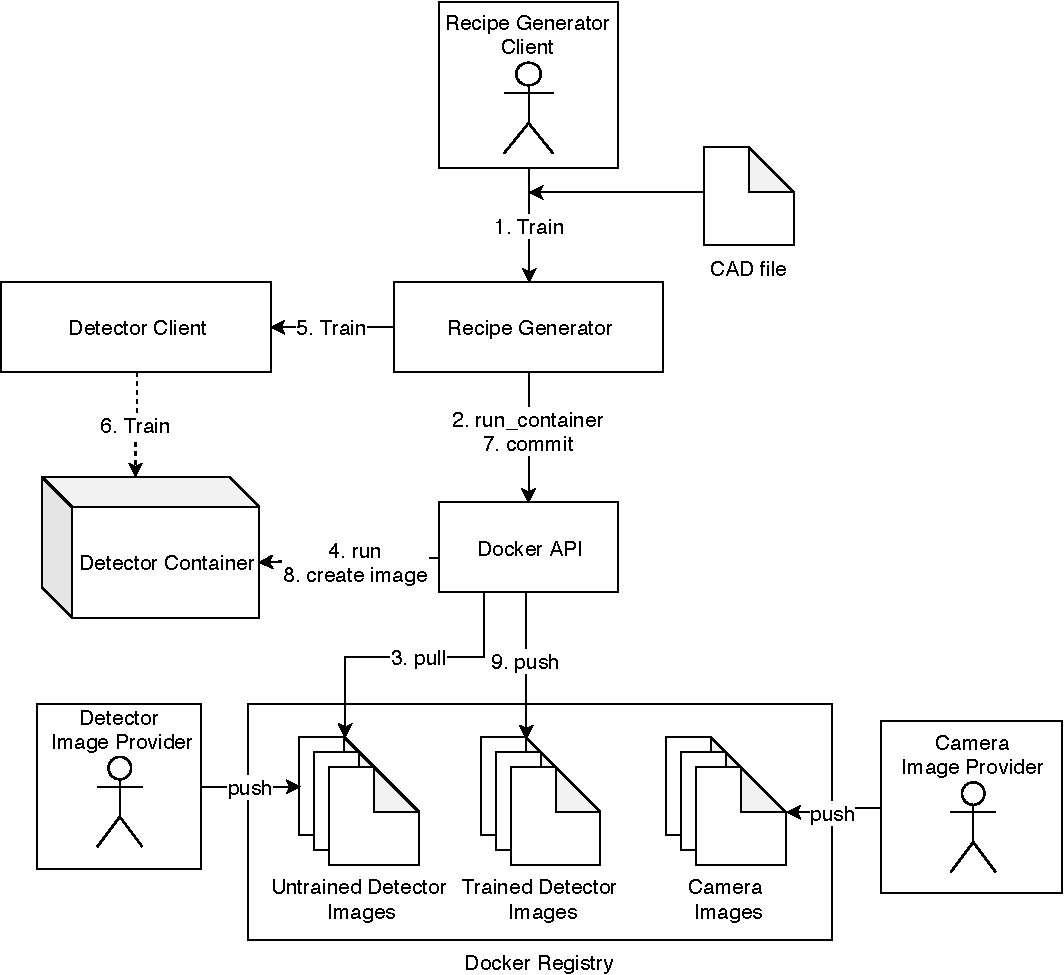
\includegraphics[width=\textwidth]{img/SequenceDiagram-Train.pdf}
	\caption{Sequence Diagram - Train}
	\label{fig:SequenceDiagram-Train}
\end{figure}

\subsection{GenRecipe} \label{subseb:genrecipe}
See figure \ref{fig:SequenceDiagram-GenRecipe}.
\mintinline{Python}{GenRecipe} takes a docker image pair (\mintinline{Python}{i}) and saves it in the recipe storage. The pair consists of one camera- and one detector docker image. As of now, the method saves the pair as a file in a folder, in the future this could be done with a database. The filename is a generated UUID later used as \mintinline{Python}{ExternalId}.
\begin{enumerate}
    \item \mintinline{Python}{GenRecipe} initializes an instance of \mintinline{Python}{Recipe} with an \mintinline{Python}{ExternalId} and calls its \mintinline{Python}{add} method.
    \begin{tabbing}
    space \= space \= spacespacespace \= spacespacespacespace \= spacespacespace \kill
    \>  GenRecipe(\\
    \>  \>  (in)	 \> 	String          \> i\\
    \>  \>  (out)	 \> 	String          \> ExternalId\\; 
    \end{tabbing}
    \item \mintinline{Python}{add} takes the image pair (\mintinline{Python}{imageList}) as input and \mintinline{Python}{write}s it into recipe/recipes folder with \mintinline{Python}{ExternalId} as filename.
    \begin{tabbing}
    space \= space \= spacespacespace \= spacespacespacespace \= spacespacespace \kill
    \>  add(\\
    \>  \>  (in)	 \> 	String          \> imageList\\;  
    \end{tabbing} \label{sign:add}
    \item \mintinline{Python}{write} writes \mintinline{Python}{imageList} as comma separated String into a file. The method is part of \mintinline{Python}{add}. \label{sign:write}
\end{enumerate}

\begin{figure}[ht]
	\centering
  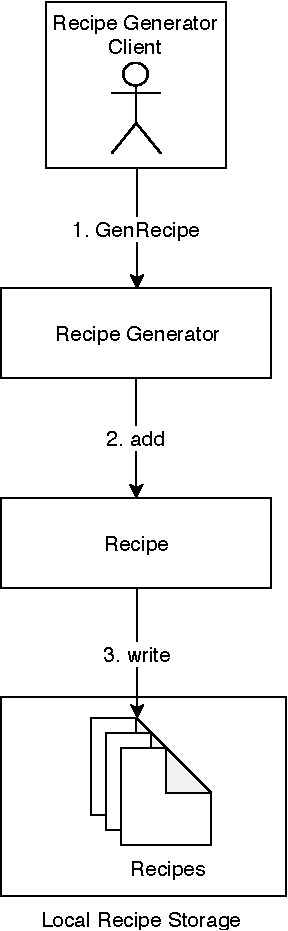
\includegraphics[height=0.5\textheight]{img/SequenceDiagram-GenRecipe.pdf}
	\caption{Sequence Diagram - GenRecipe}
	\label{fig:SequenceDiagram-GenRecipe}
\end{figure}

\subsection{Transfer}
\mintinline{Python}{Transfer} fetches the recipe and transmits it over to the OPC UA Vision server recipe management. The server has to be running for a successful method call. In the demo implementation, the recipe storage of the recipe generator and the OPC UA Vision server are the same (see \ref{fig:SequenceDiagram-Transfer}). A recipe is a pair of docker image names, the list being decorated with an \mintinline{Python}{ExternalId}. The OPC UA Vision client can be a PLC or a human machine operator. See figure \ref{fig:SequenceDiagram-Transfer}.

\begin{enumerate}
    \item \mintinline{Python}{Transfer} instantiates an instance of \mintinline{Python}{Recipe} with \mintinline{Python}{extid} and transfers the gathered image list via an OPC UA Client to the server.
    \begin{tabbing}
    space \= space \= spacespacespace \= spacespacespacespace \= spacespacespace \kill
    \>  Transfer(\\
    \>  \>  (in)	 \> 	String          \> extid\\
    \>  \>  (out)	 \> 	String          \> ExternalId; 
    \end{tabbing} \label{sign:Transfer}
    \item See point \ref{sign:Transfer}.
    \item 
    \begin{tabbing}
    space \= space \= spacespacespace \= spacespacespacespace \= spacespacespace \kill
    \>  get\_recipe(\\
    \>  \>  (out)	 \> 	Array          \> imageList; 
    \end{tabbing}
    \item 
    \begin{tabbing}
    space \= space \= spacespacespace \= spacespacespacespace \= spacespacespace \kill
    \>  add\_recipe(\\
    \>  \>  (in)	 \> 	String          \> ExternalId\\
    \>  \>  (in)	 \> 	Array          \> imageList\\
    \>  \>  (out)	 \> 	String          \> Result ; 
    \end{tabbing}\label{sign:addrecipe}
    \item OPC UA Client opens a TCP connections to OPC UA Server and then calls \mintinline{Python}{AddRecipe}. See point \ref{sign:addrecipe} for the signature.
    \item See point \ref{sign:add} in subsection \ref{subseb:genrecipe}.
    \item See point \ref{sign:write} in subsection \ref{subseb:genrecipe}.
\end{enumerate}

\begin{figure}[ht]
	\centering
  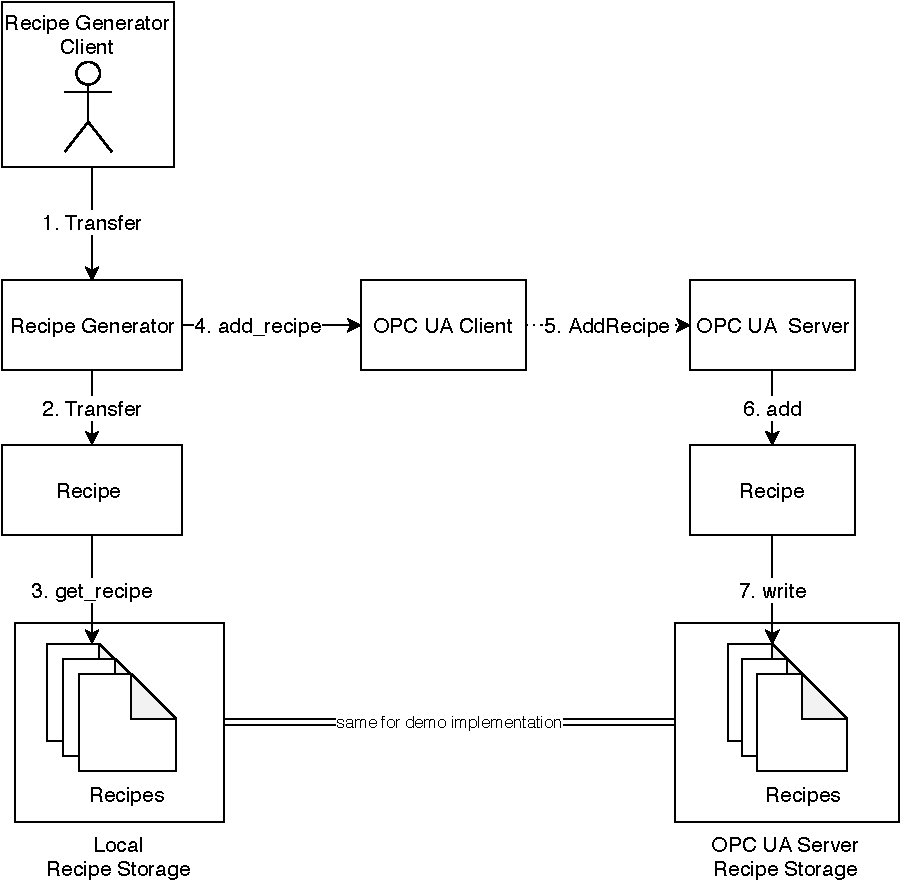
\includegraphics[width=0.7\textwidth]{img/SequenceDiagram-Transfer.pdf}
	\caption{Sequence Diagram - Transfer}
	\label{fig:SequenceDiagram-Transfer}
\end{figure}

\subsection{Prepare}
\mintinline{Python}{Prepare} runs the two docker images defined by \mintinline{Python}{ExternalId} returns. See figure \ref{fig:SequenceDiagram-Prepare}.

\begin{enumerate}
    \item 
    \begin{tabbing}
    space \= space \= spacespacespace \= spacespacespacespace \= spacespacespace \kill
    \>  PrepareRecipe(\\
    \>  \>  (in)	 \> 	String          \> ExternalId\\
    \>  \>  (out)	 \> 	String          \> Result ; 
    \end{tabbing}
    \item OPC UA Server imports the same \mintinline{Python}{Recipe} class as the recipe generator. It instantiates an instance of the class and calls the prepare method.
    \item From here onward the process is analog to the methods described before.
\end{enumerate}

\begin{figure}[ht]
	\centering
  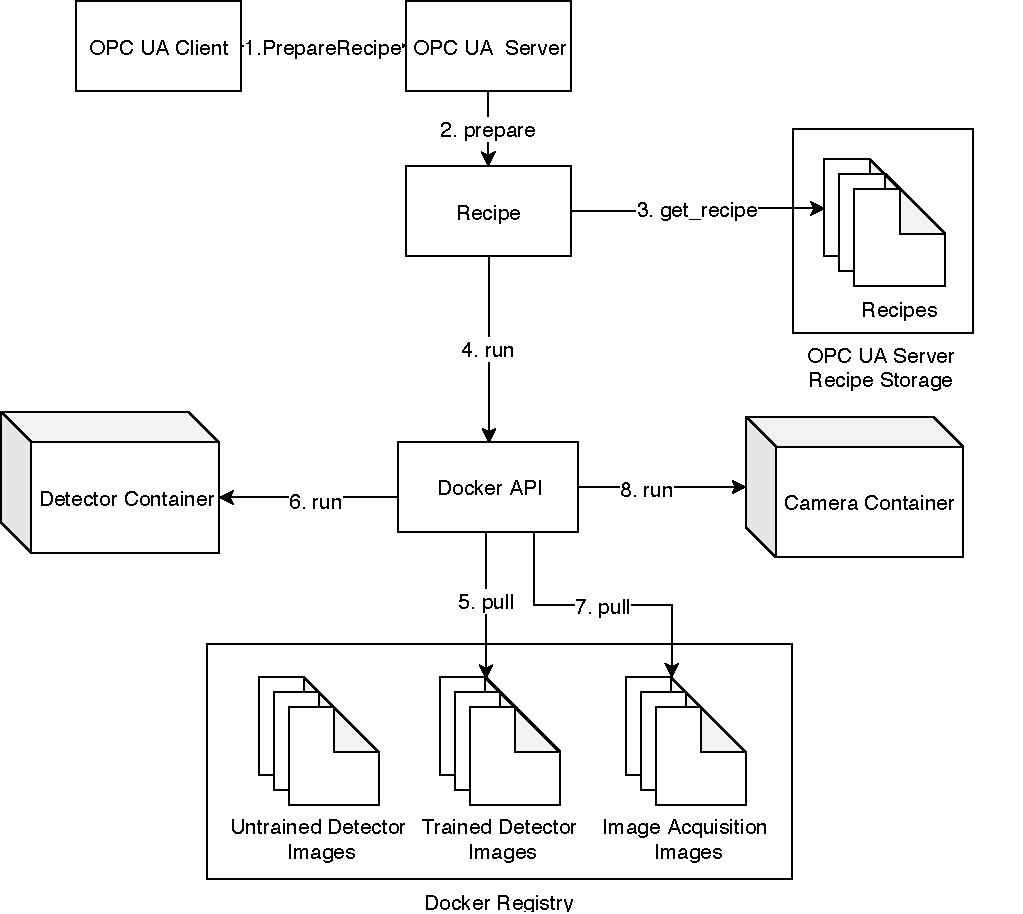
\includegraphics[width=0.7\textwidth]{img/SequenceDiagram-Prepare.pdf}
	\caption{Sequence Diagram - Prepare}
	\label{fig:SequenceDiagram-Prepare}
\end{figure}

\subsection{Test}
See figure \ref{fig:SequenceDiagram-Test}.

\begin{enumerate}
    \item OPC UA Vision server creates a \mintinline{Python}{JobId} unique for this job and returns it along with the result.
    \begin{tabbing}
    space \= space \= spacespacespace \= spacespacespacespace \= spacespacespace \kill
    \>  StartSingleJob(\\
    \>  \>  (in)	 \> 	String          \> RecipeId\\
    \>  \>  (out)	 \> 	Dict          \> Pose \\
    \>  \>  (out)	 \> 	String          \> JobId ; 
    \end{tabbing}
    \item 
    \begin{tabbing}
    space \= space \= spacespacespace \= spacespacespacespace \= spacespacespace \kill
    \>  GrabImage(\\
    \>  \>  (out)	 \> 	bytes          \> image ; 
    \end{tabbing} \label{sign:grabimage}
    \item The camera client calls the camera container located on a camera or camera image storage to fetch and return a camera image. See point \ref{sign:grabimage} for the signature.
    \item \mintinline{Python}{Test} uses the grabbed image of point \ref{sign:grabimage} to call detector client's \mintinline{Python}{Test} method. \mintinline{Python}{Test} optionally returns images to illustrates its result. 
    \begin{tabbing}
    space \= space \= spacespacespace \= spacespacespacespace \= spacespacespace \kill
    \>  Test(\\
    \>  \>  (in)	 \> 	bytes          \> image\\
    \>  \>  (out)	 \> 	Dict          \> Pose \\
    \>  \>  (out)	 \> 	bytes          \> image \\
    \>  \>  (out)	 \> 	String          \> JobId ; 
    \end{tabbing}\label{sign:Test}
    \item See point \ref{sign:Test}.
\end{enumerate}

\begin{figure}[ht]
	\centering
  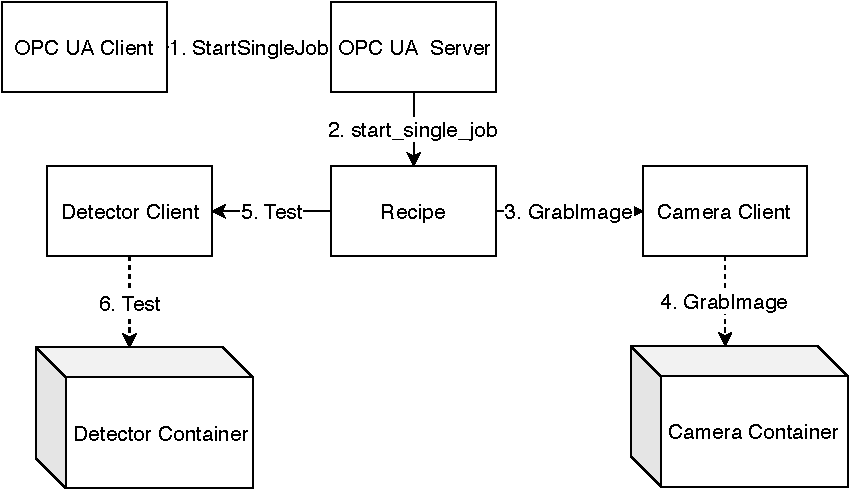
\includegraphics[width=0.7\textwidth]{img/SequenceDiagram-Test.pdf}
	\caption{Sequence Diagram - Test}
	\label{fig:SequenceDiagram-Test}
\end{figure}

\section{Class Diagram}
See figure \ref{fig:Classes} for an illustration of the used classes in the demo implementation.
\begin{figure}[h]
	\centering
  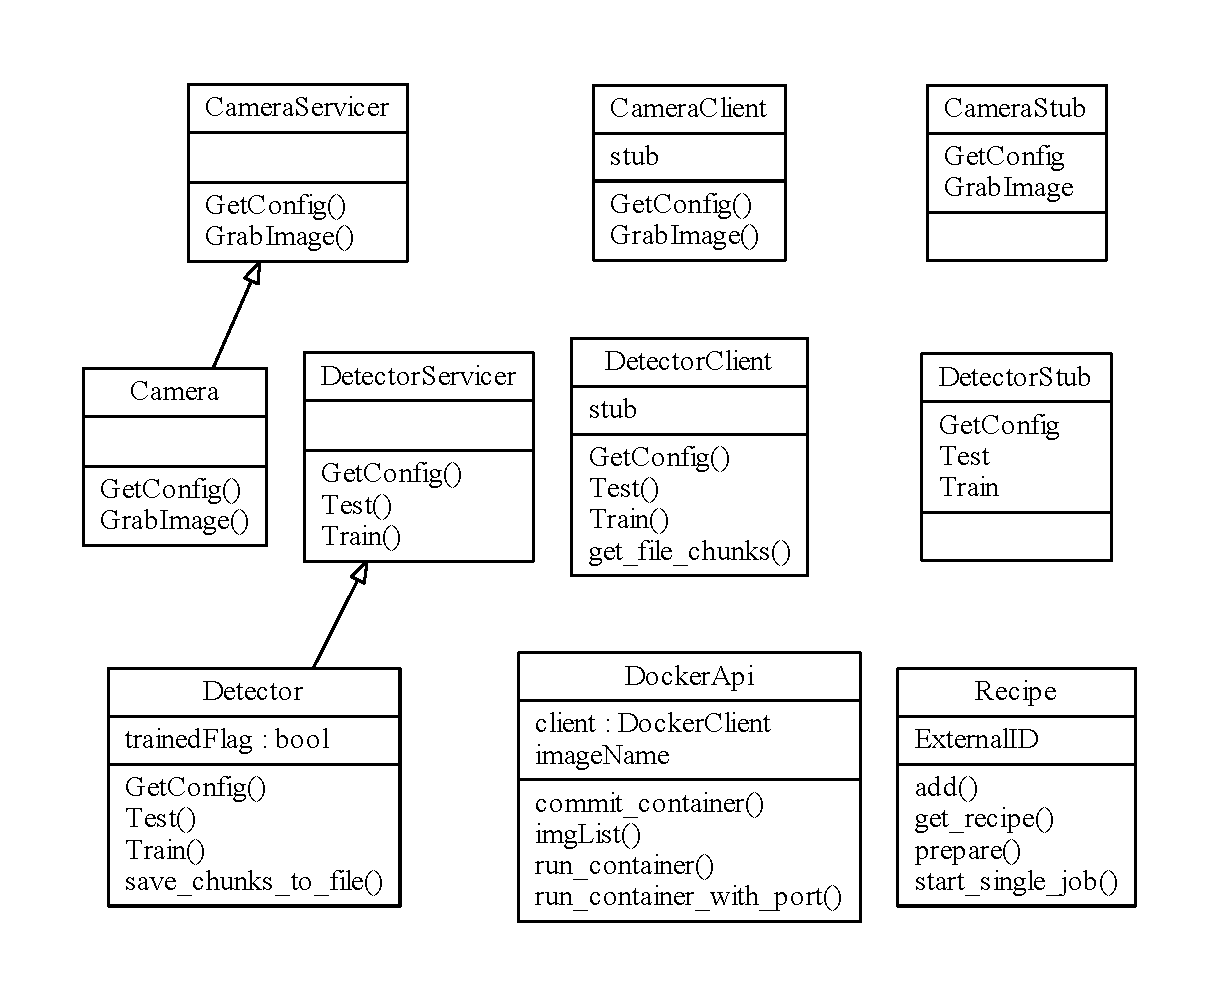
\includegraphics[width=0.9\textwidth]{img/classes.pdf}
	\caption[Class diagram]{Class diagram. Arrows denote inheritance.}
	\label{fig:Classes}
\end{figure}

\section{Package Diagram}
See figure \ref{fig:Packages} for an illustration of the used packages in the demo implementation.
\begin{figure}[h]
	\centering
  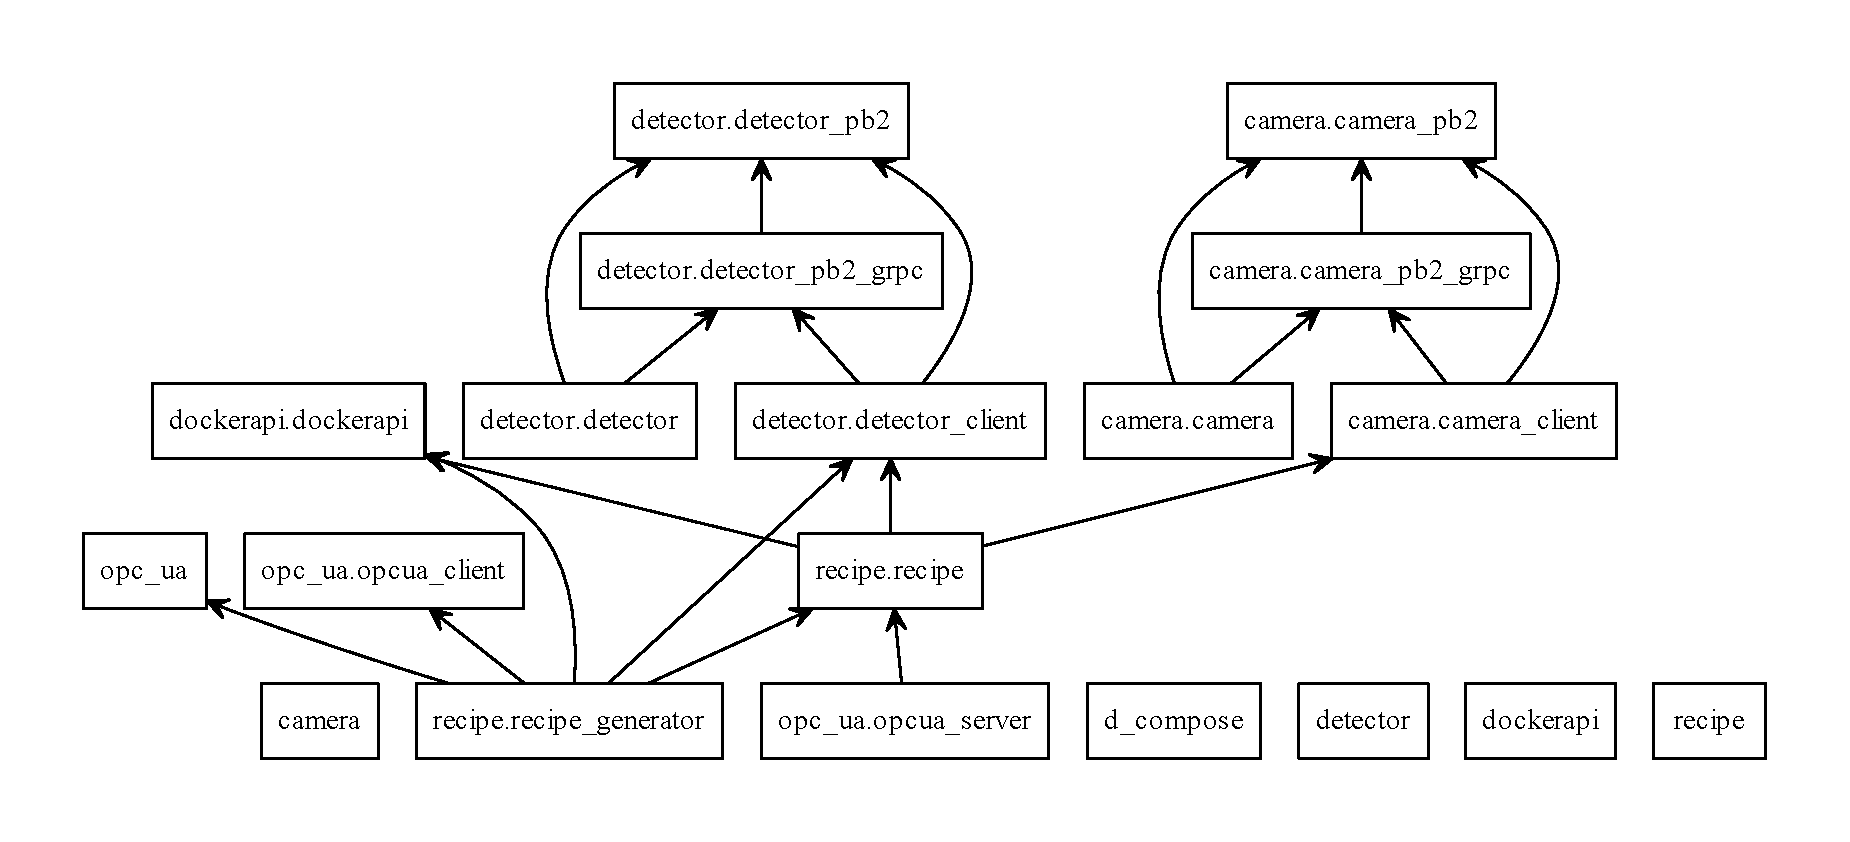
\includegraphics[width=\textwidth]{img/packages.pdf}
	\caption[Package diagram]{Package diagram. Arrows denote imports.}
	\label{fig:Packages}
\end{figure}

\section{Virtualization Technology: Docker}
\subsection{Pro}
Realizing a SOA calls for means of decoupling the components and efficient tooling. Docker is the technology which was used here due to following reasons:
\subsubsection{Dependencies of Components are handled smoothly} 
Every docker image can pull the packages and system variables it needs as specified in the dockerfile. E.g. one detector may depend on openCV 2.7.1 while another detector depends on 1.8. Both docker images that are built using their respective dockerfile are independent of each other. If no virtualization technology would be used here, a dependency handling for the whole recipe management would be necessary. In the case of two openCV versions just a slight modification of the framework may be necessary. A more drastic example would be detectors that rely on different .NET frameworks which might not be able to coexist on a system.
\subsubsection{Platform Independency}
 A platform in this context means operating system, e.g. Windows or Linux. The independency is twofold. Firstly, the docker engine runs on Linux (CentOS, Debian, Fedora, Oracle Linux, RHEL, SUSE and Ubuntu) and Windows Server. In an industrial context, both platforms are present and should be supported for maximum flexibility.
\subsubsection{Orchestration}
 Containers can be scaled if more resources are needed, monitoring and load balancing is possible and the network over which the containers communicate can be configured. See e.g. Mandy Waite's contribution to DevFest Ukraine in 2015 for more information. \cite{Waite2015ScalableContainers}
\subsubsection{Docker Hub}
 Docker offers (semi)-public or private repositories. They can be used by detector or camera providers to push their docker images and for the recipe management to pull them. As base image there are preconfigured environments available. For this implementation a fully functioning python environment was used as base docker image. To prevent know-how leaking of detection methods the accessibility to the images on the hub can be restricted. In this implementation a local repository was used with full accessibility to the docker images.
 \subsubsection{Calculations on Graphical Processing Unit}
 Some detectors need excessive calculation power. If applicable, the graphical processing unit of the bare metal server the docker engine is running on can be added. It should be kept in mind that with this technique the detector docker image is dependent not only on the docker engine but also the bare metal hardware. Thus, this option should be used with caution and only if needed.
\subsection{Contra}
\subsubsection{Lock In}
The reason against using Docker is making all involved parties introduced in \ref{sec:involvedparties} use docker. Camera and detector docker image providers need to add a dockerfile for building the image and pushing it to the repository. On the recipe management side a docker engine compatible infrastructure has to be provided. 

\section{Detector and Camera Communication: gRPC}
\subsection{Pro}
To implement the methods defined in \ref{detectormethods} gRPC was used due to following reasons: 
\subsubsection{Simple Service Definition}
In proto files you can find the service RPCs and input / output types defined. With protoc, the protocol buffer compiler, it is possible to generate place holder for clients and servers, called stubs. These place holders are the base for every camera or detector docker image provider. For a complete overview of the created proto files see \ref{proto}. 
\subsubsection{Multilingual}
Idiomatic stubs, i.e. client and server placeholders can be generated in 12 languages.\cite{LastvisitedMay4th20192019GRPCDocumentation} This is a great advantage for every provider - since no wrappers or complete rewriting of code in a possibly unknown language has to be done.
\subsubsection{Backwards Compatibility}
According to Sam Newman it is crucial to be able to deploy new servers without having to deploy clients at the time or otherwise dependently. (\cite{Newman2015BuildingMicroservices}, page 79) This is easily done with gRPC and proto3 syntax - as long as no fields are deleted or the numbers change, older clients will still be able to work with new servers.
\subsubsection{REST Gateway}
gRPC's ecosystem offers a protobuf / JSON gateway. \cite{2018-11-242017Grpc-gateway} With annotations in the proto file mappings can be set. Example from official documentation is provided here for a better understanding. Without annotations:

\begin{lstlisting}[language=protobuf3,style=protobuf]
syntax = "proto3";
package example;
message StringMessage {
  string value = 1;
}

service YourService {
  rpc Echo(StringMessage) returns (StringMessage) {}
}
\end{lstlisting}

With annotations:

\begin{lstlisting}[language=protobuf3,style=protobuf]
 syntax = "proto3";
 package example;
+
+import "google/api/annotations.proto";
+
 message StringMessage {
   string value = 1;
 }

 service YourService {
-  rpc Echo(StringMessage) returns (StringMessage) {}
+  rpc Echo(StringMessage) returns (StringMessage) {
+    option (google.api.http) = {
+      post: "/v1/example/echo"
+      body: "*"
+    };
+  }
 }
\end{lstlisting}

In the current implementation this is not done. Note that as of today, it is not supported to send files via the gateway, so a conversion of bytes to string has to be done. 
\subsubsection{Streaming}
gRPC supports HTTP/2. Especially for large files this is an advantage because multiplexed, bi-directional streams are supported. This allows for high performant file transfer. In this implemention, a byte stream was used for the Train method of the detector. See \ref{proto} for the proto file and \ref{sec:grpcpython} for an example python implementation.

\subsection{Contra}
\subsubsection{Lock In}
As well as for Docker as virtualization technology gRPC might mean extra work for detector and camera providers. Although stubs can be provided, developers still need to adhere to the service definition in the proto file.
\subsubsection{Networks will fail}
According to Sam Newman networks can never be trusted. (\cite{Newman2015BuildingMicroservices}, page 76) So, appropriate fail mechanisms have to be provided. For example, a buffering of messages is possible in case of a corrupt gRPC channel. This is not implemented in the demo framework yet.

\subsection{Stub Ports}
In the current implementation the ports on which the detector and camera server listen is static. Detectors listen on port 8000, cameras on port 8011. 

\section{Programming Language: Python}
For implenting a proof of the concept created in \ref{cha:chapter3}, a programming language supporting the components Docker, gRPC and OPC UA is highly beneficial. Python not only fulfills all three requirements, but it is also the one of the author's highest expertise.

\subsection{Support for Docker}
There is a Docker SDK available: A Python library for the Docker Engine API. It lets you do anything the docker command does, but from within Python apps – run containers, manage containers, manage Swarms, etc. \cite{LastvisitedMay4th2019DockerPython}
\begin{minted}{python}
import docker

client = docker.from_env()

# You can now run containers:
client.containers.run("ubuntu", "echo hello world")
\end{minted}

\subsection{Support for gRPC}
\label{sec:grpcpython}
Python is one of the supported languages as it is binded to gRPC's C core.  \cite{LastvisitedMay4th20192019GRPCDocumentation} Hence it is easy for the recipe generator to import necessary gRPC stubs. The gRPC client can then establish the channel. We can now call the server as shown here with the Train method:

\begin{minted}[breaklines]{python}
# detector/detector_client.py

import grpc
# import stubs containing classes and methods generated from proto file
import detector_pb2
import detector_pb2_grpc


class DetectorClient:
    def __init__(self):
        # establish a channel based on a TCP http/2 connection
        channel = grpc.insecure_channel("localhost:8000")
        # stub can be used to invoke gRPC methods
        self.stub = detector_pb2_grpc.DetectorStub(channel)
    
    def Train(self, cadFile, **kwargs):
        config = kwargs.setdefault("config", io.StringIO("dummy config"))
        # generate an iterable object of the cadFile and config
        # types have to be the same as message types in the proto file
        requestiterator = self.get_file_chunks(cadFile, config)
        # call Train method and print result
        response = self.stub.Train(requestiterator)
        print("Detector client received Train result: {0} \nAnd image: {1}".format(response.Result, response.Image))
        
# ...
\end{minted}

\subsection{Support for OPC UA}
There is an open source Python SDK for OPC UA. \cite{LastvisitedMay4th2019OPCPython} Hence it is easy for the recipe generator to import necessary OPC UA client, whilst the OPC UA client can easily connect to a server:
\begin{minted}{python}
# opcua/opcua_client.py

from opcua import Client
from opcua import ua

run():
    # populate adress space, invoke methods...

if __name__ == "__main__":
    # ...
    client = Client("opc.tcp://localhost:4840/freeopcua/server/")
    run()
\end{minted}

In the given example, the \_\_main\_\_ method is illustrated, this is of course only executed if the script is run directly and not via an import.

\section{Object Detection Methods used}
As for the demo framework implementation, only dummy detection methods were used. However, the transfer of camera images has been tested successfully.

\section{Differences to OPC UA Vision Specification}
There are major simplifications made of the OPC UA Vision specification. This is mostly due to the fact that there was no XML nodeset released by the time of implementation. The nodeset would have enabled me to import the entire information model to an OPC UA server. The following sections describe the necessary simplifications in more detail.

\subsection{Recipe Transfer}
Since the OPC UA Vision server and the recipe generator share their recipe storage and docker registry, it is sufficient to transfer the ExternalId with no additional content required. This might not be the case in a productive environment, where the topology does not allow sharing the same storage and registry. If they share at least the docker registry, then it is possible to reprogram the ExternalId to a string of concatenated docker image names, e.g. detector:latest-camera:latest. If they share none of the two, then additional image content transfer via OPC UA has to be done or the OPC UA Vision server docker registry needs to be managed externally.

\subsection{State Machine and asynchronous Methods}
According to the OPC UA Vision specification, StartSingleJob is an asynchronous method which triggers recipe execution and the state machine to transit from Ready to SingleExecution (see \ref{fig:OPCStateMachineAutomatic} and \ref{fig:runtimeviewexec}). The entire state machine of the OPC UA Vision server was neglected due to time restrictions of the thesis. As a workaround, all methods were implemented synchronously. In consequence the event containing the detection result is not sent but instead the pose is directly returned by StartSingleJob.


